\documentclass[11pt]{article}

%bibliography
\usepackage{natbib}
\bibpunct[:]{(}{)}{,}{a}{}{,}

% phonological examples

% fonts
\usepackage[normalem]{ulem}
\usepackage[T1]{fontenc}
%\usepackage{mathspec}
%\setmainfont[Mapping=tex-text]{Linux Libertine}
%\setmathfont(Digits,Greek,Latin){Linux Libertine}
%\usepackage{microtype}
%\usepackage{coptic}

\usepackage{setspace}

% tables and figures
\usepackage{booktabs}
\usepackage{floatrow}
\usepackage{enumitem}
\setlist{noitemsep}
\usepackage{multirow,sectsty}
\usepackage{subfigure,graphicx}

% Add packages and definitions you want to use here:
\usepackage[papersize={8.5 in, 11 in}, nohead, left=1.5 in, right = 1 in, vmargin= 1 in]{geometry}

%\usepackage{times}


%\usepackage{tipa}

\usepackage{amssymb}
\usepackage[all]{xypic}


% titles
\title{Prepositional Case, Incorporation and Nominative Recipient Passives}
\author{Hezekiah Akiva Bacovcin}

\usepackage{gb4e}
\noautomath

\begin{document}
\maketitle
\section{Outline}
\begin{enumerate}
	\item Background and Theory
	\item Evidence from History of English
	\item Evidence from Swedish
\end{enumerate}

\section{Background and Theory}
Main claim of dissertation: \textbf{All recipients are base generated as prepositional dative phrases in the specifier of an applicative phrase} (Dative PP + applicative analysis):

\begin{exe}
	\ex Applicative Analysis (with dative PP):\\
			\xymatrix@=2pt{
			& ApplP\ar@{-}[dl]\ar@{-}[dr]\\
			PP_{\text{Recipient}} & & \bar{Appl}\ar@{-}[dl]\ar@{-}[dr]\\
			& Appl & & VP\ar@{-}[dl]\ar@{-}[dr]\\
			& & DP_{\text{Theme}} & & \bar{V}\ar@{-}[d]\\
			& & & & V}
\end{exe}

Theme--recipient orders (e.g., ``I gave the books to John'') are created by scrambling the theme into a higher specifier of the applicative \citep{McGinnis.1998}

\xymatrix@=2pt{
 & vP\ar@{-}[dl]\ar@{-}[dr]\\
DP\ar@{-}[d] & & \bar{v}\ar@{-}[dl]\ar@{-}[dr]\\
\text{Mary} & \text{v} & & ApplP\ar@{-}[dl]\ar@{-}[dr]\\
 & & DP\ar@{-}[d] & & \bar{Appl}\ar@{-}[dl]\ar@{-}[dr]\\
 & & \text{the book$_{i}$}\ar@{<-}@(dl,dl)[ddrrr] & DP\ar@{-}[d] & & \bar{Appl}\ar@{-}[dl]\ar@{-}[dr]\\
 & & & \text{to John} & Appl & & VP\ar@{-}[dl]\ar@{-}[dr]\\
 & & & & & DP_{i} & & \bar{V}\ar@{-}[d]\\
 & & & & & & & V}
 

Following \cite{Bayer.2001} and \cite{Asbury.2005,Asbury.2007}, inherent case is represented syntactically as a preposition heading a prepositional phrase (dative PP). Other prepositional phrases (e.g., goals) are distinguished by both featural content in the head of the preposition and position within the clause (applicative vs. object of the verb).

\begin{exe}
	\ex Prepositional Object Construction:\label{ex:POC} \\
\xymatrix@=2pt{
	& VP\ar@{-}[dl]\ar@{-}[dr] \\
 DP_{\text{Theme}} && \bar{V}\ar@{-}[dl]\ar@{-}[dr]\\
 &  V & & PP_{\text{Goal}}}
\end{exe}

Structural case (e.g., nominative and accusative) are properties of DPs and crucially not PPs \citep{Bayer.2001}.\footnote{I am deliberately being agnostic between a dependent case and classical case theory as to how nominative and accusative case are assigned. As far as I can tell, all of my claims are compatible with both frameworks.} 

\textbf{Problem:} How do we get nominative recipient passives (e.g., ``He was given the book.'')?

\textbf{Proposed Solution:} P-incorporation! \citep{Alexiadou.2014}

\textbf{Assumption 1:} P-incorporation (or more properly P-excorporation) moves the P-head out of the PP (details discussed with motivating data below).

\textbf{Assumption 2:} Phrases rely on the presence of their head (removal the head $\rightarrow$ removal of phrase)

\textbf{Conclusion:} Recipients whose dative P head has excorporated become bare DPs (and thus available for receiving nominative case, e.g., nominative recipient passives)

\begin{exe}
	\ex \textbf{Forshadowing:} Should see evidence of P-incorporation elsewhere
	\begin{xlist}
		\ex Evidence of nominative passivisation in Dutch and German
		\ex Pseudopassivisation and nominative recipient passivisation in history of English
		\ex Swedish prefix verbs
	\end{xlist}
\end{exe}
\section{Evidence from German and Dutch}

\cite{Alexiadou.2014} motivate their P-incorporation analysis with data from German and Dutch.

With the normal passive auxiliary (\textit{werden} `become') only theme passives are possible:
\begin{exe}
	\ex High German:\label{ex:hg-normal-pass}
\begin{xlist}
	\ex[ ]{\gll Ich glaube, dass \textbf{den} \textbf{Kindern} das Fahrrad geschenkt worden ist.\\
	I beleive that \textbf{the.DAT.PL} \textbf{children} the.NOM bicycle granted become be.3sg\\
\trans `I believe that the children were granted the bicycle.'}
\ex[*]{\gll Ich glaube, dass \textbf{die} \textbf{Kindern} das Fahrrad geschenkt worden sind.\\
I beleive that \textbf{the.NOM.PL} \textbf{children} the.ACC bicycle granted become be.3pl\\
\trans `I believe that the children were granted the bicycle.'}
\end{xlist}
\ex Dutch:\label{ex:dutch-normal-pass}
\begin{xlist}
	\ex[ ]{\gll De boeken \textbf{werden} haar aangeboden.\\
		the books \textbf{became.PL} her given\\
	\trans `The books were given to her.' \citep[ex. 5b]{Broekhuis.1994}}
	\ex[*]{\gll Zij \textbf{werd} de boeken aangeboden.\\
	she.NOM \textbf{became.SG} the books given\\
	\trans `She was given the books.' \citep[ex. 5c]{Broekhuis.1994}}
\end{xlist}
\end{exe}

However, when a different auxiliary is used, (the equivalent of the GET-passive) nominative recipients are possible:

\begin{exe}
	\ex High German:\label{ex:hg-get-pass}
\begin{xlist}
	\ex \gll dass der Vater \textbf{der} \textbf{Tochter} ein Buch geschenkt hat\\
	that the.NOM father \textbf{the.DAT} \textbf{daughter} a.ACC book sent has\\
	\trans `that the father sent the daughter a book.'
	\ex \gll dass \textbf{die} \textbf{Tochter} von dem Vater ein Buch geschenkt bekommen hat\\
	that \textbf{the.NOM} \textbf{daughter} by the father a.ACC book sent got has\\
	\trans `that the daughter got sent a book by her father \cite[183]{Draye.1996}.'
\end{xlist}
\ex Dutch:\label{ex:dut-get-pass}
\gll \textbf{Zij} kreeg de boeken (van mij) aangeboden.\\
\textbf{she.NOM} got the books (by me) given\\
\trans `She was given the books (by me).' \citep[ex. 7]{Broekhuis.1994}
\end{exe}

According to \cite{Alexiadou.2014}, the different auxiliary reflects contextual allomorphy in the passive auxiliary based on the presence or absence of the dative P.

\newpage
\section{Evidence from History of English}

	\begin{figure}[t!]
		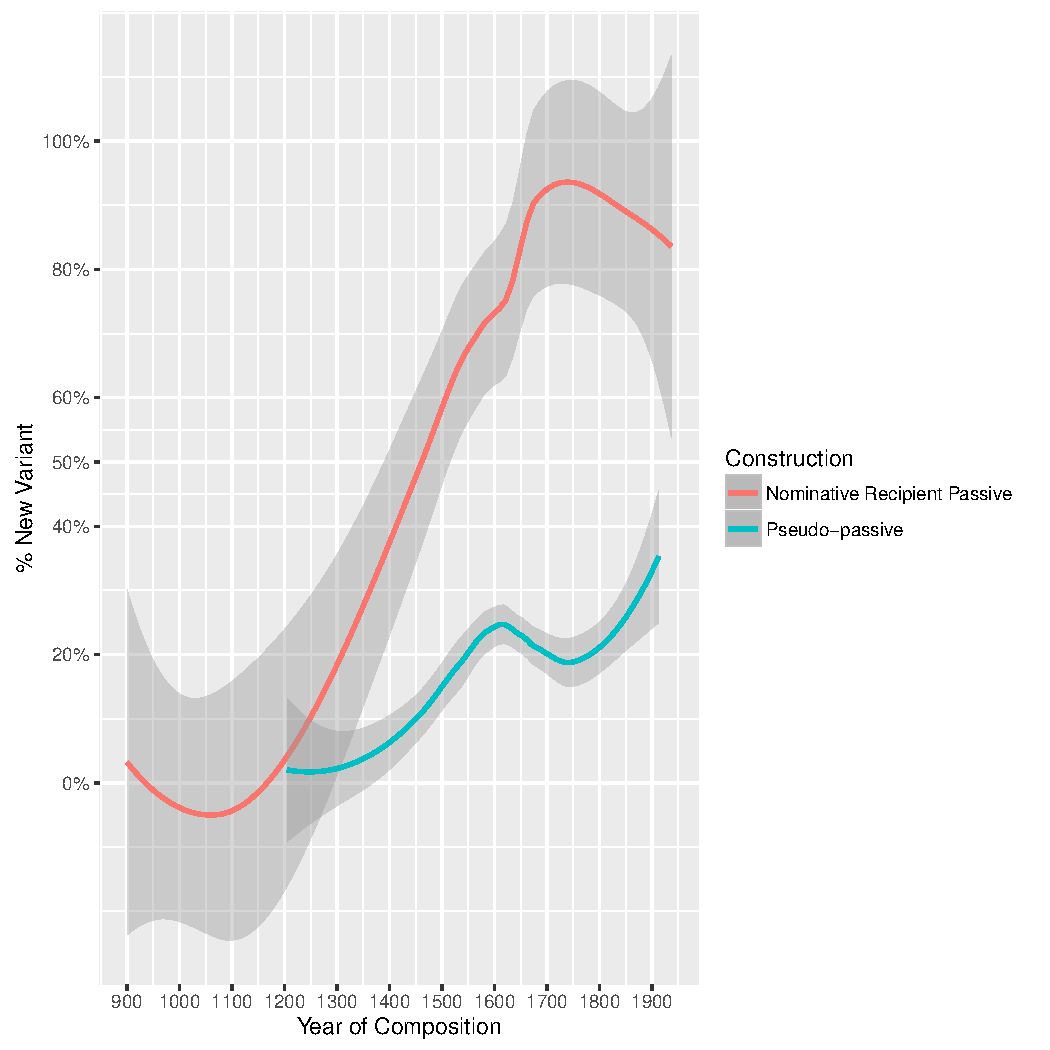
\includegraphics[width=\linewidth]{../images/recpas-pseudo}
		\caption{Logistic regression curves showing rates of nominative recipient passivisation and pseudopassivisation in English}
		\label{fig:recpas-pseudo}
	\end{figure}


Pseudopassivisation (e.g., ``The bed was slept in'') has also been proposed to be derived via P-incorporation \citep{Herslund.1984}

In English, pseudopassivisation and nominative recipient passivisation enter the language at the same time and show a Constant Rate Effect (only suggestive due to small data on recipient passivisation). See Figure \ref{fig:recpas-pseudo}.


\section{Evidence from Swedish}
Swedish has two different classes of ditransitive verbs that behave differently in both active and passive contexts. The prefixed verbs can be derived via P-incorporation of the dative P into the verbal stem. Thus, these ``words'' always require P-incorporation to occur \citep{Holmberg.1995}.

\begin{exe}
	\ex Crucial data points (data below):
	\begin{xlist}
		\ex Only unprefixed verbs can occur in theme--recipient order in active
		\ex Only prefixed verbs can have recipient passives, which are nominative recipient passives
	\end{xlist}
\end{exe}
\begin{exe}
	\ex Theoretical Conclusions:
	\begin{xlist}
		\ex P-incorporation blocks the theme from scrambling (would be intervener between recipient and main verb for P-incorporation)
		\ex Again, P-incorporation licenses nominative recipient passivisation (but also maybe bare theme passivisation???)
	\end{xlist}
\end{exe}

\textbf{Structural definition of P-incorporation:} P-incorporation moves the P-head from the specifier of the recipient -- itself in the specifier of the applicative phrase -- and adjoins it to the head of the nearest C-commanding phrase.

Here is an example tree:
\begin{exe}
\ex P-incorporation (VO Word Order)\label{ex:VO-Pincorp}\\
			\xymatrix@=2pt{
			& VoiceP\ar@{-}[dl]\ar@{-}[dr]\\
			V+Appl+Voice\ar@{<-}[dd] && ApplP\ar@{-}[dl]\ar@{-}[drr]\\
			& PP_{\text{Recipient}}\ar@{-}[dl]\ar@{-}[dr] & & & \bar{Appl}\ar@{-}[dl]\ar@{-}[dr]\\
			\text{\sout{P}} & & DP_{\text{Recipient}} & \text{\sout{Appl}} & & VP\ar@{-}[dl]\ar@{-}[dr]\\
			&  &  &  & \text{\sout{V}} & & DP_{\text{Theme}}}
\end{exe}

The relevant Swedish data for discussion:

\subsubsection{Relevant Citations}
\cite{Haugen.1982,Falk.1990,Falk.1993,Holmberg.1995,Falk.1997,Anward.1989,Holmberg.2002,Lundquist.2004,Platzack.2005,Lundquist.2006,Bardal.2007,Lundquist.2013,Lundquist.2013b,Haddican.2014,Haddican.2015}
\subsubsection{Active Data}
\begin{exe}
	\ex Swedish:
		\gll Jag gav Johan en bok.\\
		I gave John a book.\\
		\trans `I gave John a book \citep{Holmberg.1995}.'
	\ex Swedish:
		\gll Jag gav en bok *(til) Johan.\\
		I gave a book to John.\\
		\trans `I gave a book to John \citep{Holmberg.1995}.'

	\ex Swedish:
			\begin{xlist}
				\ex \gll Han gav Jan bollen\\
				he.NOM gave John ball.the\\
				\trans `He gave John the ball'
				\ex \gll Han gav bollen *(til) Jan\\
				he.NOM gave ball.the to John\\
				\trans `He gave the ball to John'
			\end{xlist}
	\ex Swedish:
			\begin{xlist}
				\ex[ ]{\gll Han erbjöd Jan ett nytt jobb\\
				he.NOM offered John a new job\\
			\trans `He offered John a new job'}
				\ex[??]{\gll Han erbjöd ett nytt jobb til Jan\\
				he.NOM offered a new job to John\\
			\trans `He offered a new job to John'}
				\ex[*]{\gll Han erbjöd ett nytt jobb Jan\\
				he.NOM offered a new job John\\
			\trans `He offered a new job to John'}
			\end{xlist}

\end{exe}
\subsubsection{Passive Data}
\begin{exe}
	\ex Swedish:
	\begin{xlist}
		\ex[ ]{Particle Verb:
		\gll Han erbjöds ett nytt jobb\\
			he.NOM offered.PASS a new job\\
			\trans `He was offered a new job (\citealt{Anward.1989}, \citealt{Lundquist.2006}).'}
		\ex[*]{Non-Particle Verb:
		\gll Pelle gavs ett äpple\\
			Pelle gave.PASS a apple\\
			\trans `Pelle was given an apple (\citealt{Anward.1989}, \citealt{Lundquist.2006}).'}
	\end{xlist}	
	\ex Swedish (verbs without particles):
		\sn[*]{
			\gll Ett äpple gavs Pelle.\\
			 An apple gave.PASS Pelle.\\
			 \trans `An apple was given to Pelle (\citealt{Anward.1989},\citealt{Lundquist.2006}).'}
	\ex Swedish:
		\gll Ett nytt jobb erbjöds=honom.\\
		A new job offered.PASS=him.OBL.\\
		\trans `A new job was offered to him (\citealt{Anward.1989},\citealt{Falk.1990},\citealt{Lundquist.2006}).'
	\ex Swedish:
		\gll *Ett äpple gavs honom.\\
		 An apple gave.PASS him.\\
		 \trans `An apple was given to him (\citealt{Anward.1989},\citealt{Lundquist.2006}).'
	 \ex Swedish:
		\gll Jobbet erbjöds mannen med den långa svarta kappan.\\
		job.DEF offered.PASS man.DEF with the long black coat\\
		'The job was offered to the man with the long black coat \citep[ex 26]{Lundquist.2004}.'
	\ex Swedish:
		\begin{xlist}
			\ex[ ]{\gll Mannen som erbjöds \textbf{jobbet} hade redan tackat ja till ett annat jobb.\\
			man.DEF who offered.PASS \textbf{job.DEF} had already thanked yes to a other job\\
			\trans `The man, who was offered the job, had already accepted another job \citep[ex. 51]{Lundquist.2004}.'}
			\ex[??]{\gll Mannen som \textbf{jobbet} erbjöds hade redan tackat ja till ett annat jobb.\\
			man.DEF who \textbf{job.DEF} offered.PASS had already thanked yes to a other job\\
			\trans `The man, to whom the job was offered, had already accepted another job \citep[ex. 52]{Lundquist.2004}.'}
		\end{xlist}
	\ex Swedish:
		\begin{xlist}
			\ex[ ]{\gll Jobbet som erbjöds \textbf{mannen} var mycket slitsamt.\\
			job.DEF which offered.PASS \textbf{man.DEF} was very tiring\\
			\trans `The job, which was offered to the man, was very tiring \citep[ex. 49]{Lundquist.2004}.'}
			\ex[ ]{\gll Jobbet som erbjöds \textbf{mannen} var mycket slitsamt.\\
			job.DEF which \textbf{man.DEF} offered.PASS was very tiring\\
			\trans `The job, which the man was offered, was very tiring \citep[ex. 50]{Lundquist.2004}.'}
		\end{xlist}
\end{exe}



\bibliographystyle{mcbride}
\bibliography{../diss}
\end{document}
